% !TEX root = main.tex

\section{贝叶斯决策论} % 2.1-2.9 (2.10-2.11)
% 贝叶斯判定
%  2.2 连续特征
%  2.3 最小误差分类
%    极小极大、Neyman-Pearson
%  2.4 分类器、判别函数、判定面
%  2.9 离散特征 x\in\{0,1\}
% 正态分布的判别函数 2.5 2.6
% 2.7 误差概率和误差积分
% 2.8 正态密度误差上界
% 2.10 丢失特征、噪声特征
% 2.11 贝叶斯置信网
% 样本均值 协方差矩阵

\subsection{贝叶斯决策}
处于类别$\sC_k$并具有特征值$\vx$,有后验概率\footnote{课本用$\omega_i$表示类别,用$p(\cdot)$代表概率密度函数(连续变量),用$P\lrp{\cdot}$代表概率质量函数(离散变量)}\textemph{(给特征判类别)}
\[p(\sC_k\mid\vx)=\frac{p(\vx\mid\sC_k)p(\sC_k)}{p(\vx)}\]
即
\[posterior=\frac{likelihood\times prior}{evidence}\]

决策域$\mR_k$使得落在其中的点都被归为类别$\sC_k$,在两个决策域的交界称为\textbf{决策边界},则平均错误概率可表示为
\[\begin{aligned}
p\lrp{error}&=p(\vx\in\mR_1,\sC_2)+p(\vx\in\mR_2,\sC_1)\\
&=\intabu{\mR_1}{}{p(\vx,\sC_2)}{\vx}+\intabu{\mR_2}{}{p(\vx,\sC_1)}{\vx}\\
&=\intabu{\mR_1}{}{p(\sC_2\mid\vx)p(\vx)}{\vx}+\intabu{\mR_2}{}{p(\sC_1\mid\vx)p(\vx)}{\vx}\\
\end{aligned}\]
注意$p(\vx)$是证据,可以看为是固定分布(常量)。

\begin{figure}[H]
\centering
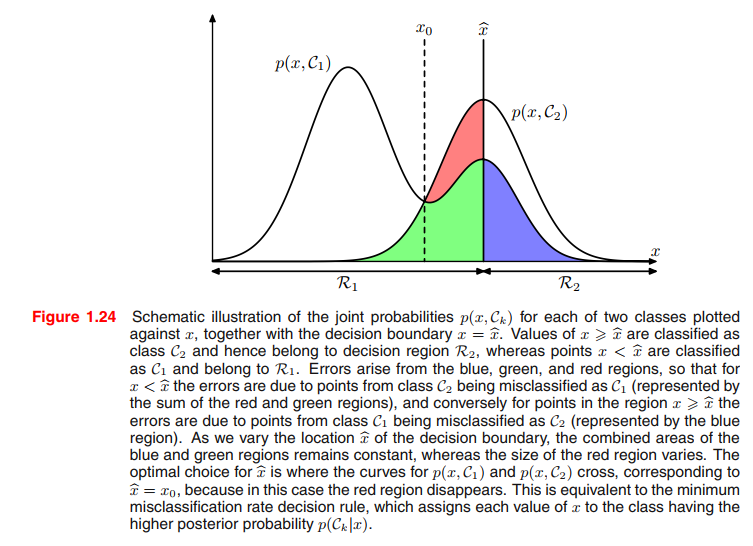
\includegraphics[width=0.8\linewidth]{fig/bayesian_decision.png}
\end{figure}
\begin{theorem}[贝叶斯决策/最小错误率准则]
若$p(\sC_1\mid \vx)>p(\sC_2\mid \vx)$,则判定类别为$\sC_1$;否则判为$\sC_2$。
或有等价判别$p(\vx\mid \sC_1)p(\sC_1)>p(\vx\mid\sC_2)p(\sC_2)$。
依照这种准则可以获得最小错误率,即
\[p(error\mid \vx)=\min [p(\sC_1\mid \vx),p(\sC_2\mid \vx)]\]
\end{theorem}

由于在现实生活中,我们的目标往往不仅是令归类错误率最小,而通常附带了权重,因此有损失函数$\lambda_{ij}$代表将正确类别$\sC_j$归为$\sC_i$的损失,则将$\vx$归到$\sC_i$的风险(risk)为
\[R_i=\sum_{j=1}^c\lambda_{ij}\lambda_{ij}p(\vx\in\sR_i,\sC_j)\]
总风险为
\[\begin{aligned}
R&=\sum_{i=1}^cR_i\\
&=\sum_i\sum_j\lambda_{ij}\int_{\sR_i}p(\sC_j\mid \vx)p(\vx)\diff x\\
&=\sum_i\int_{\sR_i}\sum_j\lambda_{ij}p(\sC_j\mid \vx)p(\vx)\diff x
\end{aligned}\]
由于$p(\vx)$为常量,故要让总风险最小化只需令每一项决策的条件风险最小化
\[R(\sC_i\mid\vx)=\sum_{j=1}^v\lambda_{ij}p(\sC_j\mid\vx)\]
此即贝叶斯决策论,最小化总的风险称为贝叶斯风险,记为$R^*$

Neyman-Pearson准则是限定某一类别$\sC_i$的风险不能超过一个常数,但会导致总的误差率提升。

\subsubsection{二类分类}
特别地,对于二类分类问题,定义对称损失/0-1损失
\[\lambda(\alpha_i\mid\omega_j)=
\begin{cases}
0 & i=j\\
1 & i\ne j
\end{cases}
\qquad i,j=1,2,\ldots,c\]
有条件风险
\[\begin{aligned}
R(\alpha_1\mid\vx)&=\lambda_{11}P(\omega_1\mid\vx)+\lambda_{12}P(\omega_2\mid\vx)\\
R(\alpha_2\mid\vx)&=\lambda_{21}P(\omega_1\mid\vx)+\lambda_{22}P(\omega_2\mid\vx)
\end{aligned}\]

可得贝叶斯决策
\[\frac{p(\vx\mid\omega_1)}{p(\vx\mid\omega_2)}>\frac{\lambda_{12}-\lambda_{22}}{\lambda_{21}-\lambda_{11}}\frac{P(\omega_2)}{P(\omega_1)}\]

\subsubsection{极小极大化准则}
有时先验$p(\vx)$并不准确,因此我们想要让最小风险尽可能小,即极小极大化准则。

\subsection{正态密度}
\begin{itemize}
	\item 连续单变量正态函数
\[p(x)=\frac{1}{\sqrt{2\pi}\sigma}\exp\lrs{-\frac{1}{2}\lrp{\frac{x-\mu}{\sigma}}^2}\thicksim N(\mu,\sigma^2)\]
有期望和方差
\[\begin{aligned}
\mu &= \E{x}=\int_{-\infty}^\infty xp(x)\diff x\\
\sigma^2 &=\E{(x-\mu)^2}=\int_{-\infty}^\infty (x-\mu)^2 p(x)\diff x
\end{aligned}\]

	\item $d$维多元高斯分布
\[p(\vx)=\frac{1}{(2\pi)^{d/2}|\Sigma|^{1/2}}\exp\lrp{-\frac{1}{2}(\vx-\vmu)^\T\Sigma^{-1}(\vx-\vmu)}\thicksim N(\vmu,\Sigma)\]
其中$\vmu$为$d$维均值向量,$\Sigma$维$d\times d$协方差矩阵,同时
\[\begin{aligned}
\vmu &=\E{\vx} = \int\vx p(\vx)\diff\vx\\
\Sigma &=\E{(\vx-\vmu)(\vx-\vmu)^\T} = \int(\vx-\vmu)(\vx-\vmu)^\T p(\vx)\diff\vx
\end{aligned}\]
每一元素为
\[\begin{aligned}
\mu_i &= \E{x_i}\\
\sigma_{ij} &= \E{(x_i-\mu_i)(x_j-\mu_j)}
\end{aligned}\]
注意协方差矩阵$\Sigma$通常是对称且半正定的。
但这里我们严格限定$\Sigma$为正定的,使得$\Sigma$的行列式是一个正数。
\end{itemize}

服从正态分布的随机变量的线性组合都是一个正态分布。
特别地,若$p(\vx)\thicksim N(\vmu,\Sigma)$,$A$是$d\times k$的矩阵,且$\vy=A^\T\vx$是一$k$维向量,则
\[p(\vy)\thicksim N(A^\T\vmu,A^\T\Sigma A)\]
协方差用于计算数据沿任何方向或任意子空间的分散程度。
\begin{figure}[H]
\centering
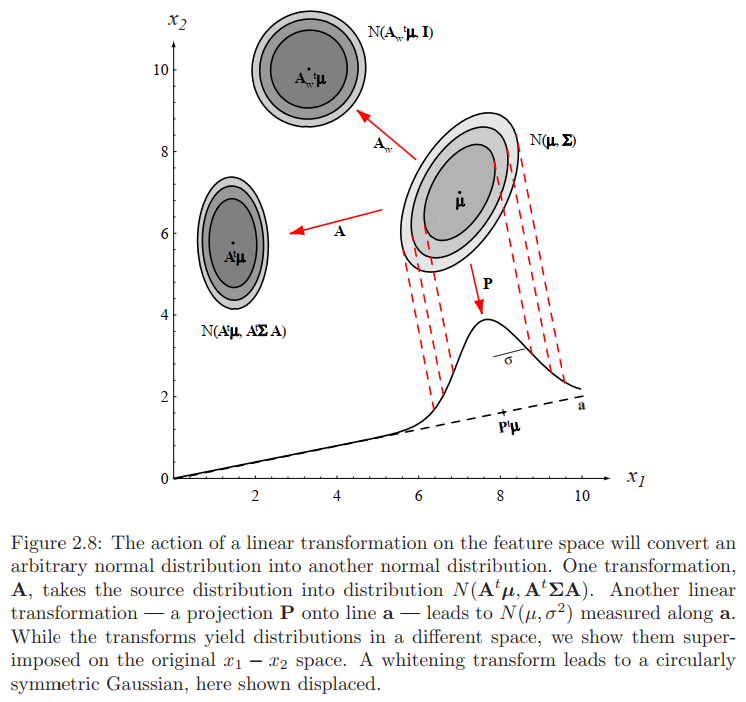
\includegraphics[width=0.8\linewidth]{fig/covariance_matrix.png}
\end{figure}

某个分布的协方差矩阵与单位阵$I$成比例,若定义矩阵$\Phi$,其列向量是$\Sigma$的正交本征向量\footnote{先求特征值和特征向量,然后将特征向量归一化},$\Lambda$为与相应本征值对应的对角矩阵,变换
\[A_w=\Phi\Lambda^{-1/2}\]
将使变换后的分布的协方差矩阵成为\textbf{单位阵}\footnote{这种表示方法是$\Cov{A_w^\T}=I$},此变换称为白化变换。

从$\vx$到$\vmu$的平方马氏(Mahalanobis)距离定义为(即正态分布中的指数部分)
\[r^2=(\vx-\vmu)^\T\Sigma^{-1}(\vx-\vmu)\]
可以证明与一Mahalanobis距离$r$对应的超椭球体体积为
\[V=V_d|\Sigma|^{1/2}r^d\]
其中$V_d$是一个$d$维单位超球体的体积
\[V_d=\begin{cases}
\pi^{d/2}/(d/2)! & d\text{为偶数}\\
2^d\pi^{(d-1)/2}\lrp{\frac{d-1}{2}}!/d! & d\text{为奇数}
\end{cases}\]
因此对于一给定维数,样本的离散程度直接随$|\Sigma|^{1/2}$而变化。

最小误差概率分类可用判别函数获得(即极大后验)
\[g_i(\vx)=\ln p(\vx\mid\omega_i)+\ln P(\omega_i)\]
如果$p(\vx\mid\omega_i)\thicksim N(\vmu,\Sigma)$,则可以求得
\[g_i(\vx)=-\frac{1}{2}(\vx-\vmu)^\T\Sigma_i^{-1}(\vx-\vmu_i)-\frac{d}{2}\ln 2\pi-\frac{1}{2}\ln|\Sigma_i|+\ln P(\omega_i)\]